\documentclass[11pt]{article}

\usepackage{graphicx, epsfig}
\usepackage{amsmath, amssymb, latexsym}
\usepackage[english]{babel}
\usepackage{amssymb}   
%\usepackage{graphicx}
%\usepackage{float} 






% Make a larger page (shrink the margins)
%
\setlength{\textwidth}{6.7in}
\setlength{\textheight}{9.0in}
\setlength{\evensidemargin}{0.0in}
\setlength{\oddsidemargin}{0.0in}
\topmargin -0.5in
\footskip 0.5in



\title{Confirming Instrument Consistency Between Sites}
\author{Eric Davis}
\begin{document}
\maketitle
\medskip



\section{Time Profiles}
\hspace{0.5cm}

As you are probably aware, I have used the Forth Smith data to locate an object consistently that could be useful for calibration. As luck would have it, Jupiter appears to satisfy the requirement that a) Its apparent magnitude changes slightly in the time frame for the data (approximately 30 days) and b) is consistently visible for the time frame of the data in the Northern hemisphere i.e. all the ground sites. 


\begin{figure}[h!]
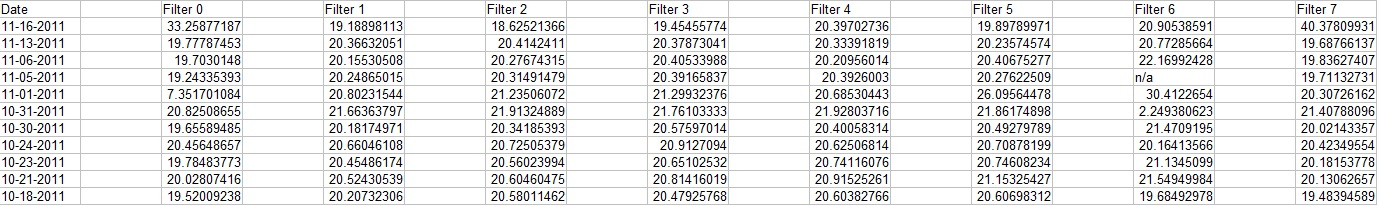
\includegraphics[scale=0.5]{fwhmcomparison.jpg}
\caption{A comparison of Jupiter's time profile over 11 different nights for the various filters. There are a couple outliers, and they are a result of artifacts in the data and should probably be ignored for any analysis performed on the data}
\end{figure}



\section{Future Considerations}

Next week I will find average values (excluding outliers) for the FWHM in each filter. From there I hope to produce a plot that will give some indication of the differences in what the photometer is picking up depending on the wavelength of light. Other important characteristics are the maximum photon counts the photometer receives, which should offer some insight into what is occurring withing the instrument itself. This data will also likely be analyzed using some type of plot


\end{document}
\end{article}